\documentclass[12pt,letterpaper]{article}

\usepackage[hypertexnames=false]{hyperref}
\usepackage{amsmath}
\usepackage{graphicx}
\usepackage{enumerate}

% Custom packages
\usepackage{amssymb}
\usepackage{booktabs}       % professional-quality tables
\usepackage{algorithm}      % algorithm environment
\usepackage{algpseudocode}
\usepackage{multirow}
\usepackage{sectsty}
\usepackage{tabularx}
\usepackage{tikz}           % vector graphics
\usepackage{bm}             % bold math symbols
\usepackage{xcolor}
\usepackage{microtype}
\usepackage{import}
\usepackage{titling}
\usepackage{natbib}
\usetikzlibrary{arrows, backgrounds, patterns, matrix, shapes, fit, 
  calc, shadows, plotmarks}


% Custom commands
\let\oldvec\vec
\renewcommand\vec{\bm}
\newcommand{\simfn}{\mathtt{sim}} % similarity function
\newcommand{\truncsimfn}{\underline{\simfn}} % truncated similarity function
\newcommand{\blockfn}{\mathtt{BlockFn}} % blocking function
\newcommand{\distfn}{\mathtt{dist}} % distance function
\newcommand{\valset}{\mathcal{V}} % attribute value set
\newcommand{\entset}{\mathcal{R}} % set of records that make up an entity
\newcommand{\partset}{\mathcal{E}} % set of entities that make up a partition
\newcommand{\1}[1]{\mathbb{I}\!\left[#1\right]} % indicator function
\newcommand{\euler}{\mathrm{e}} % Euler's constant
\newcommand{\dblink}{\texttt{\upshape \lowercase{d-blink}}} % Name of scalable Bayesian ER model
\newcommand{\blink}{\texttt{\upshape \lowercase{blink}}} % Name of original Bayesian ER model
\def\spacingset#1{\renewcommand{\baselinestretch}%
  {#1}\small\normalsize} \spacingset{1}

\newtheorem{remark}{Remark}
\newtheorem{proposition}{Proposition}
\newtheorem{definition}{Definition}
\newtheorem{lemma}{Lemma}
\def \brian#1{{\color{red} (#1)}}
\def \serge#1{{\color{blue} (#1)}}
\def \beka#1{{\color{green} (#1)}}

% DON'T change margins - should be 1 inch all around.
\addtolength{\oddsidemargin}{-.5in}%
\addtolength{\evensidemargin}{-.5in}%
\addtolength{\textwidth}{1in}%
\addtolength{\textheight}{1.3in}%
\addtolength{\topmargin}{-.8in}%

\sectionfont{\large\nohang\centering\MakeUppercase}

\title{Bayesian Matching with Relaxed Duplication Assumptions through Dirchlet Record Linkage}
\author{Brian Kundinger}

\begin{document}
\maketitle
%
%\bigskip
\begin{abstract}
	Probabilistic record linkage is the use of statistical methods to identify unique entities within and across databases. Bayesian methods can adopt different prior distributions for various assumptions on the nature of record duplications in the linkage task, but become computationally expensive as the size of the linkage task grows. In this paper, we propose Dirichlet Record Linkage (\texttt{DRL}),	a method for linking duplicate-free reference file to target file that may have internal duplications. We use a Dirichlet prior for the parameter governing the number of matches a record in the reference file has in the target file. We decompose this parameter into a sequence of conditional probabilities, and use these parameters in a computationally efficient Gibbs sampler to conduct the linkage task. We demonstrate the speed and accuracy of our method relative to other recent Bayesian methods through simulations and case studies. In particular, we show that \texttt{DRL} exhibits strong performance using default, noninformative hyperparameters.  
\end{abstract} 

%
%\newpage
\spacingset{1.5}

%\section{Introduction}


%\section{Review of fabl}
%
%The full model for fabl is given by:
%
%\begin{subequations}
%	\begin{align}
%		\mathcal{L}(Z, \bm{m}, \bm{u} \mid \gamma) &= \prod_{i=1}^{n_A}  \prod_{j=1}^{n_B}\prod_{f=1}^{F}\prod_{l=1}^{L_f}\left[  m_{fl}^{I(Z_j = i)}u_{fl}^{I(Z_j \neq i)}\right]^{I(\gamma_{ij}^f = l)I_{obs}(\gamma_{ij}^f)}, \label{eqn:likelihood}\\
%		\bm{m}_f &\sim \text{Dirichlet}(\alpha_{f1}, \ldots, \alpha_{f L_f}), \forall f = 1, \ldots, F, \label{eqn:m} \\
%		\bm{u}_f &\sim \text{Dirichlet}(\beta_{f1}, \ldots, \beta_{f L_f}),\forall f = 1, \ldots, F,  \label{eqn:u}\\
%		p(Z_j = q| \pi)  &=
%		\begin{cases} 
%			\frac{1}{n_A}\pi,  & q > 0; \\
%			1-\pi, &  q  = 0; \\
%		\end{cases} \label{eqn:z}\\
%		\pi &\sim \text{Beta}(\alpha_{\pi}, \beta_{\pi})\label{eqn:pi}.
%	\end{align}
%\end{subequations}

%\section{Motivation}
%
%We have shown in previous work that the fast Beta linkage framework tends to outperform standard Fellegi Sunter when each record in $B$ has at most one match in $A$. However, significant problems arise when a record in $B$ has multiple matching records in $A$. In particular, since matching probability is normalized among all records in $A$, matching probability is split among multiple records such that none of the matches achieves high enough posterior probability to be identified through the Bayes estimate. This amounts to a paradox: the more matches that record $B_j$ has in $A$, the less likely the algorithm is to find a match. 
%
%We attempt to resolve this paradox by extending the fabl framework to handle these internal duplications. We introduce a modified Dirichlet process prior that allows each record in $B$ to match to potentially multiple records in $B$. We emphasize that we are not interested in deduplication within either dataset for its own sake, but rather aim to conduct record linkage in light the problems posed by these duplications. For this reason, we do not enforce transitive closure throughout the Gibbs sampler as done in \cite{marchant_distributed_2019} and \cite{aleshinguendel2021multifile}, but rather assume it, and create a coherent set of linkages through post-processing. This allows for a record linkage model that is robust to internal duplications while maintaining the computational advantages of the original \texttt{fabl} model.


\newpage

\section{Introduction}\label{sec:introduction}

%We have shown in previous work that the fast Beta linkage framework tends to outperform standard Fellegi Sunter when each record in $B$ has at most one match in $A$. However, significant problems arise when a record in $B$ has multiple matching records in $A$. In particular, since matching probability is normalized among all records in $A$, matching probability is split among multiple records such that none of the matches achieves high enough posterior probability to be identified through the Bayes estimate. This amounts to a paradox: the more matches that record $B_j$ has in $A$, the less likely the algorithm is to find a match. 

%We attempt to resolve this paradox by extending the fabl framework to handle these internal duplications. We introduce a modified Dirichlet process prior that allows each record in $B$ to match to potentially multiple records in $A$. We emphasize that we are not interested in deduplication within $A$ for its own sake, but rather aim to conduct record linkage in light the problems posed by these duplications. Therefore, duplications within files that have no duplications across files will go undetected; we believe this acceptable for many practical applications. 

 %For this reason, we do not enforce transitive closure throughout the Gibbs sampler as done in \cite{marchant_distributed_2019} and \cite{aleshinguendel2021multifile}, but rather assume it, and create a coherent set of linkages through post-processing. This allows for a record linkage model that is robust to internal duplications while maintaining the computational advantages of the original \texttt{fabl} model.

%There have been several other attempts to estimate more flexible linkage structures within the comparison vector framework, but each has significant drawbacks in practice. First, the original \cite{fellegi_theory_1969} method that models the linkage status of each record pair as independent typically results in one record in one file being matched with multiple records in the other file. This initial estimate of the linkage structure is usually refined through post-processing to create a bipartite matching \cite{jaro1989}. As of yet, this post-processing has not been adapted to estimate more general linkage structures, and the initial estimate without any post-processing is known to have poor precision. \cite{aleshin2023multifile} allowed for multiple matches within and across datafiles, but requires that the modeller explicitly set a maximum linkage cluster size, and models the dependency between records in such a way that limits scalability. 
Probabilistic record linkage is the use of statistical methods to identify unique entities within and across databases, generally without the use of unique identifiers. This is an increasingly important task in ``data cleaning,'' either for its own sake, or as a preliminary step before conducting subsequent analysis. These techniques are used in government, non-profit organizations, healthcare, industry, and their use continues to grow. \citep[e.g.,][]{Herzog_2007, christen_data_2012, Papadakis2021, binette2022almost}. In this paper, we propose a method for conducting record linkage between a duplicate free reference file and some other file that may have internal duplications. 

%It is common for data collectors to have one list of records with a rigorous sampling mechanism trusted to have no internal duplications, or have to cleaned a list over time such 

Many probabilistic record linkage methods are based on the foundational work of \cite{fellegi_theory_1969}. In these Fellegi-Sunter (FS) methods, the data analyst first creates comparison vectors for each pair of records in the data files. These vectors indicate how similar the records are on a set of variables measured in both files, known as the linkage variables.  Using these comparison vectors, the analyst classifies each pair as a match or nonmatch using a likelihood ratio test. An alternative paradigm is to model the linkage variables directly \citep[e.g.,][]{tancredi2011hierarchical, steorts_bayesian_2016, marchant_distributed_2019, betancourt2022prior}. In this article, we build on the contributions to the comparison vector approach.

In the original FS formulation, record pairs are independently classified as matches or nonmatches, but through a  Bayesian framework, practitioners can formalize different assumptions on the type of matchings between files through different prior distributions on the linkage structure. For example, \cite{sadinle_bayesian_2017} proposed prior distribution on one-to-one matchings between two files, and \cite{aleshin2023multifile} proposed a prior on the partitions of records corresponding to unique entities found in arbitrarily many files. These more tailored record linkage methods have the advantage of producing coherent sets of matches that respect transitivity without the need for post-processing, but have limited scalability. 

Much work has been done to expand the the scalability of FS methods. One approach is to reduce the number of comparisons vectors needed for analysis through ``blocking'', using some feature in the data to allocate records into smaller partitions (or blocks), and running linkage algorithms independently on each block \citep{christen2019data}. Of note, blocking on an unreliable field can lead to missed matches, making this form of blocking often undesirable \citep{steorts_comparison_2014}. Others use ``filtering'', which uses some deterministic or probabilistic criteria to set the match probability for certain comparison vectors to zero after they have been created \citep{murray2016probabilistic, mcveigh2019scaling}. In the creation of the \texttt{fastLink} method, \cite{enamorado2019using} formalized the use of a lower dimensional representation of the set of comparison vectors that allowed for much faster parameter estimation of the standard FS model; \cite{kundinger_2023} and \cite{kundinger_2024_vabl} then adopted this approach for a faster implementation of the bipartite model of \cite{sadinle_bayesian_2017}.
 
In this work, we continue this work of proposing new record linkage methods tailored for important practical scenarios, and the computational methods to implement them in an efficient and scalable manner. We introduce Dirichlet Record Linkage (\texttt{DRL}, pronounced ``drill"), an extension of the comparison vector record linkage framework for the scenario of linking one duplicate-free reference file to another file with unknown amounts of internal duplications. To do so, we model the parameter governing the amount of matches between files as Dirichlet process. Since the resulting set of possible matches for each record is extremely high dimensional, we propose an innovative Gibbs sampler utilizing the stick-breaking represenation of the Dirichlet process for tractable posterior inference. We adopt the dimension reduction techniques of \cite{kundinger_2023} for additional gains in speed and scalability. 

In what follows, Section~\ref{sec:prior-work} reviews the work of \cite{fellegi_theory_1969} and a selection of Bayesian extensions to contextualize our intervention. Section~\ref{sec:drl} introduces \texttt{DRL}, and describes our approach for efficient posterior sampling. Sections~\ref{sec:simulations} and \ref{sec:case-study} demonstrate the speed and accuracy of our method in relation to several other comparison vector techniques in a series of simulations a case study of voter registration records in North Carolina. Finally, Section~\ref{sec:conclusion} summarizes our work and discusses areas for further research.

%Crucially, these decisions are made independently for each pair. The \cite{fellegi_theory_1969} approach has been extended for a wide variety of applications \citep[e.g.,][]{Winkler1990, fair2004generalized, wagner2014person, gill2003english, enamorado2019using, aleshinguendel2021multifile}. 


%First, the original \cite{fellegi_theory_1969} method that models the linkage status of each record pair as independent typically results in one record in one file being matched with multiple records in the other file. This initial estimate of the linkage structure is usually refined through post-processing to create a bipartite matching \cite{jaro1989}. As of yet, this post-processing has not been adapted to estimate more general linkage structures, and the initial estimate without any post-processing is known to have poor precision.

%\cite{aleshin2023multifile} allowed for multiple matches within and across datafiles, but requires that the modeller explicitly set a maximum linkage cluster size, and models the dependency between records in such a way that limits scalability. 



\section{The Fellegi-Sunter Framework for Record Linkage}\label{sec:prior-work}

Consider two data files $A$ and $B$ comprising $n_A$ and $n_B$ records, respectively, and including $F$ linkage variables measured in both files. For $i=1, \dots, n_A$, let record $i$ be given by $A_i = (A_{i1}, \dots, A_{iF})$, so that $A = (A_i : i = 1, \dots, n_A)$.  Similarly, for $j=1, \dots, n_B$, let record $j$ be given by $B_j = (B_{j1}, \dots, B_{jF})$, so that $B = (B_j : j = 1, \dots, n_B)$. 

In record linkage tasks, records that refer to the same entity should be similar, and records that refer to different entities should be dissimilar. To represent this, \cite{fellegi_theory_1969} proposed using the comparison vector $\gamma_{ij} = (\gamma_{ij}^1, \ldots, \gamma_{ij}^F),$ where $\gamma_{ij}^f$ is a comparison for field $f$ between records $A_i$ and $B_j$. Binary comparisons are commonly used due to their simplicity; partial agreement or more complicated comparisons can be used through similarity metrics or distance functions \citep{Winkler_1990, Bilenko_2003_adapt, elmagarmid_duplicate_2007}. We assume that each field's comparison is discretized , and we let $L_f$ denote the number of categories for field $f$. We collect all of the comparison vectors as $\gamma=\{\gamma_{ij}\}_{i=1,j=1}^{n_A,n_B}$.

Consider records from $A$ and $B$ as disjoint set of nodes. We have an edge between two records if they are coreferent (or matching). Our parameter of interest is the collection of edges representing coreferent records. This parameter can be expressed in various ways depending on the model assumptions for a particular approach to record linkage. For example, \cite{fellegi_theory_1969} used a coreferent matrix $\Delta \in \{0, 1\}^{n_A \times n_B}$, where
\begin{align}
	\Delta_{ij} =
	\begin{cases}
		1, & \text{if records}\;  A_i \; \text{and}\; B_j \; \text{refer to the same entity}; \\
		0, & \text{otherwise}.\\
	\end{cases}
\end{align}
This sparse matrix representation can become cumbersome for large linkage tasks. In the setting where each record in $B$ can match to at most one record in $A$, \cite{sadinle_bayesian_2017} proposed using the more compact vector $\bm{Z} = (Z_1, \ldots, Z_{n_B})$ for the records in $B$ such that
\begin{align}
	Z_{j} =
	\begin{cases}
		i, & \text{if records}\;  A_i \; \text{and}\; B_j  \; \text{refer to the same entity}; \\
		n_A + j, & \text{if record}\;  B_j \; \text{does not have a match in}\; A. \\
	\end{cases}
\end{align}

\subsection{Models for Comparison Vector Based Record Linkage}\label{sec:model-review}

For modeling the collection of $n_An_B$ random variables $\Gamma_{ij}$, \cite{fellegi_theory_1969} employ two independence assumptions: first, that comparison vectors are independent given the matching status of the record pair, and second, that the matching status of each record pair is independent of the matching status of other pairs. Using these independence assumptions, one specifies a mixture model for each $\Gamma_{ij}$ \citep[e.g., as in ][]{winkler_state_1999,jaro1989,larsen_2001,enamorado2019using}.  We have
\begin{subequations}
	\begin{align}
		&\Gamma_{ij} \mid \Delta_{ij} = 1 \stackrel{iid}{\sim} \mathcal{M}(\bm{m}), \label{eqn:fs_model} \\
		&\Gamma_{ij} \mid \Delta_{ij} = 0  \stackrel{iid}{\sim} \mathcal{U}(\bm{u}), \label{eqn:m_dist}\\
		&\Delta_{ij}   \stackrel{iid}{\sim} \text{Bernoulli}(\lambda). \label{eqn:lambda_dist}
	\end{align}
\end{subequations}
Here, $\mathcal{M}$ and $\mathcal{U}$ are the distributions for matching and nonmatching record pairs, $\bm{m}$ and $\bm{u}$ are their respective sets of parameters, and $\lambda$ is the marginal probability that a record pair is a match. When using comparison vectors with discrete agreement levels, $\mathcal{M}$ and $\mathcal{U}$ are collections of independent multinomial distributions for each linkage feature. Accordingly, $\bm{m} = (\bm{m}_1, \ldots, \bm{m}_F)$, where $\bm{m}_f = (m_{f1}, \ldots, m_{fL_f})$ and $m_{fl} = p(\Gamma_{ij}^f = l|\Delta_{ij} = 1)$ for all fields $f$ and agreement levels $l$. The $\bm{u}$ parameters are defined similarly, with $u_{fl} = p(\Gamma_{ij}^f = l|\Delta_{ij} = 0)$.

One advantage of Bayesian methods is the ability to use prior distributions tailored to specific model assumptions, which tends to produce better results than post-processing after using more general methods. Under the assumption that there are no duplicates within files, \cite{sadinle_bayesian_2017} proposed the ``beta distribution for bipartite matching,'' given by
\begin{align}
	\mathbb{P}(Z\mid \pi) &=\dfrac{[n_1-n_{12}(Z)]!}{n_1!} %\times
	\pi^{n_{12}(Z)}(1-\pi)^{n_2-n_{12}(Z)},  	\label{eq:brlprior}\\
	\pi &\sim \text{Beta}(\alpha_{\pi}, \beta_{\pi}).
\end{align}
This prior induces a Gibbs sampler that strictly enforces one-to-one matching, and has has been shown to outperform the base FS method when model assumptions are satisfied. However, maintaining the dependencies between records has limited this method to small to moderate linkage tasks.

More recently, \cite{aleshin2023multifile} extended the FS framework for the setting of arbitrary amount of duplications within and across an arbitrary number of files. To do so, they presented a generative process for multifile partitions, and parameterized each step of this generative process. This leads to a structured prior for multifile partitions consisting of
\begin{enumerate}
	\item A prior for the number of unique entities exhibited in the linkage task. By default, this is taken to be uniform over total number of records in the linkage task.
	\item Given the total number of unique entities, a prior for the \emph{overlap table}, or the number of unique entities exhibited in each file. This prior is given by a multinomial-Dirichlet distribution.
	\item Given the number of unique entities exhibited in each file, a prior for the number of records in each file associated with each unique entity. By default, this is taken to be a Poisson distribution truncated between 1 and the number of records in each file.
	\item Given the number of records in each file associated with each unique entity, a prior for the within-file partitions of records to entities. This is taken to be uniform over the number of such assignments.
	\item Given the overlap table and within-file partitions, a prior for the matching between files. This is taken to be uniform over all possible such matchings. 
\end{enumerate}
To our knowledge, this is as of yet the only comparison vector method that can identify duplicates within files with out employing the full record pair independence from the original \cite{fellegi_theory_1969}. This structured prior induces a Gibbs sampler on the partition of records corresponding to the unique entities in the record linkage task. Similarly the beta prior for bipartite matching however, this Gibbs sampler becomes infeasible for larger linkage tasks. 

\subsubsection{Fast Beta Linkage}\label{sec:fabl}

\cite{kundinger_2023} proposed to model each element of $Z$ independently, relaxing the assumption that there are no duplicates within each database. Under this relaxation, they introduced the fast beta linkage (\texttt{fabl}) prior:
\begin{align}
	\mathbb{P}(Z_j = i \mid \pi) 
	&=
	\begin{cases}
		\pi/n_1,  &  \text{if}  \; i\leq n_1,\\
		1- \pi, &   \text{if}  \;  i= n_1 + j,
	\end{cases}\label{eqn:fabl} \\
	\pi &\sim \text{Beta}(\alpha_{\pi}, \beta_{\pi}) \label{eqn:pi_beta},
\end{align}
where $\alpha_{\pi}, \beta_{\pi}$ are fixed and known. This prior says that a record $B$ has some match in $A$ with probability $\pi$, and that each record in $A$ is equally likely to be that match. The \texttt{fabl} prior closely mimics the beta prior for bipartite matchings in \eqref{eq:brlprior}, without enforcing the bipartite matching restriction within the Gibbs sampler. This prior was originally proposed for an efficient Gibbs sampler, but was recently shown to be estimable through variational inference for substantial computational gains \citep{kundinger_2024_vabl}. If desired, a bipartite matching can be acquired through a simple post-processing step after computing the Bayes estimate. 



\section{Dirichlet Record Linkage}\label{sec:drl}

We showed in \cite{kundinger_2023} and \cite{kundinger_2024_vabl} that the \texttt{fabl} framework tends to outperform standard FS when each record in $B$ has at most one match in $A$. However, significant problems arise when a record in $B$ has multiple matching records in $A$. In particular, since matching probability is normalized among all records in $A$, matching probability is split among multiple records such that none of the matches achieves high enough posterior probability to be identified through the Bayes estimate. This amounts to a paradox: the more matches that record $B_j$ has in $A$, the less likely the algorithm is to find a match. Here, we attempt to resolve this paradox by extending the \texttt{fabl} framework to handle these internal duplications in $A$. We emphasize that we are not interested in deduplication within $A$ for its own sake, but rather aim to conduct record linkage in light the problems posed by these duplications. Therefore, duplications within files that have no duplications across files will go undetected; we believe this acceptable for many practical applications. 

We provide updated notation to allow us to describe matching in this setting. Let $Z_j = (Z_{j, 1}, \ldots)$ be a set containing the indices for all of the records in $A$ that are a match with record $B_j$, and let $Z = \{Z_j | j = 1, \ldots, n_B\}$ denote the collection of such sets for all records in $B$. Let $|Z_j|$ denote the number of records in $A$ that are linked to $B_j$. We use $Z_j = \emptyset$ to denote when $B_j$ has no match in $A$. 

%Recall that for \texttt{fabl}, we used the following prior for the linkage structure $Z$ and the rate of matching parameter $\pi$:
%\begin{subequations}
%	\begin{align}
	%		p(Z_j = q| \pi)  &=
	%		\begin{cases} 
		%			\frac{1}{n_A}\pi,  & q > 0; \\
		%			1-\pi, &  q  = 0; \\
		%		\end{cases} \label{eqn:fabl_prior}\\
	%		\pi &\sim \text{Beta}(\alpha_{\pi}, \beta_{\pi})\label{eqn:pi_beta}.
	%	\end{align}
%\end{subequations}
% We now generalize these prior distributions to allow the records in $B$ to match with multiple records in $A$. 

%In this section, we relax the assumption of no duplicates within either file, and allow for duplicates within one file. We adapt the ideas behind \texttt{fabl} to propose an efficient and scalable method for this setting. In particular, we generalize the prior distribution provided in \eqref{eqn:fabl} and \eqref{eqn:pi_beta} to allow the records in $B$ to match with multiple records in $A$. 

%We introduce a Dirichlet process prior that allows each record in $B$ to match to potentially multiple records in $A$. We emphasize that we are not interested in deduplication within $A$ for its own sake, but rather aim to conduct record linkage in light the problems posed by these duplications. Therefore, duplications within files that have no duplications across files will go undetected; we believe this acceptable for many practical applications. 



Define a vector of probabilities $\bm{\pi} = (\pi_0, \ldots)$ where $\pi_k$ is the probability that some record $B_j$ has exactly $k$ matches in $A$. To avoid setting a maximum number of matches for any $B_j$, we assign $\bm{\pi}$ a Dirichlet process prior. That is, 
\begin{align}\label{eqn:pi-dirichlet-process}
	f(\bm{\pi}) = \sum_{k=0}^{\infty} \pi_k \delta_{\pi_k}(\bm{\pi}),
\end{align}
where $\delta_{\pi_k}$ is the indicator function which evaluates to zero everywhere, except for $\delta_{\pi_k}(\pi_k) = 1$. We model each $\pi_k$ as a product of conditional probabilities: let $\eta_k$ be the probability that some record in $B$ has at least $k$ matches, given that it has at least $k-1$ matches. This gives us the stick breaking representation
\begin{align}\label{eqn:pi-stick-breaking}
	\pi_k = (1 - \eta_{k+1}) \prod_{c=1}^{k} \eta_c, 
\end{align}
where $\eta_k$ are independent random variables from a $\text{Beta}(1, \beta_{\eta})$ distribution.

Conditional on $B_j$ having $k$ matches, we construct a prior specification on $Z$ such that each matching $Z_j$ of length $|Z_j|$ is equally likely. Since there are ${n_A \choose |q|} = \frac{n_A!}{(n_A - |q|)! |q|!}$ ways to select $|q|$ matching records out of all $n_A$ possible records, we use
\begin{align}
	p(Z_j = q| \bm{\pi}) = \frac{(n_A - |q|)! |q|!}{n_A!} \pi_{|q|}. \label{eqn:z_drl}
	%\bm{\pi} \sim \text{Dirichlet}(\alpha_{\pi}) \label{eqn:pi_drl}.
\end{align}
In Appendix~\ref{app:joint-distribution}, we show that the full conditional for $Z_j$ in this setting is given by
\begin{align}
		p\left(Z_j  = q|\gamma, \bm{m}, \bm{u}, \pi \right) \propto \frac{(n_A - |q|)!|q|!}{n_A!} \pi_{|q|} \prod_{i \in q} w_{ij}, \label{eqn:joint_posterior}
\end{align}
where for all $i \in \{1, \ldots, n_A\}$ and $j \in \{1, \ldots, n_B\}$, 
\begin{align}
	w_{ij} = \prod_{f=1}^{F}\prod_{l = 1}^{L_f} \left(\frac{m_{fl}}{u_{fl}}\right)^{I(\gamma_{ij}^f = l)I_{obs}(\gamma_{ij}^f)} \label{eqn:fs_weight}.
\end{align}

Finally, to obtain an estimate $\hat{\bm{Z}}$ of the linkage structure, we use the loss functions and Bayes estimate from \cite{sadinle_bayesian_2017} and adapted by \cite{kundinger_2023}. Since (\ref{eqn:z_drl}) does not strictly enforce the requirement that there are no duplicates in $B$, it is possible for this Bayes estimate to link multiple records in $B$ to the same record in $A$. To obtain a Bayes estimate that corresponds to our model assumptions, we minimize the expected loss subject to the constraint that $\hat{Z}_{j, k} \neq \hat{Z}_{j', k}$ for all $j \neq j'$ and all $k$. See Supplement \ref{app:bayes-estimate} for details regarding this initial Bayes estimate and this post-processing procedure.

\subsection{Sequential Sampler}\label{sec:sequential-sampler} 

Sampling the full conditional in (\ref{eqn:joint_posterior}) is infeasible for almost any record linkage task. In particular, there are $2^{n_A}$ possible matchings for each $B_j$, meaning that computational complexity for the sampler would be $O\left(n_B 2^{n_A}\right)$. One could reduce this computational burden by setting a maximum number of matches, $K$, per record in $B$, but this would still require $\sum_{k = 1}^K \frac{n_A!}{(n_A - k)!k!}$ possible options for the set $Z_j$, and would be prohibitive for most values of $n_A$ seen in record linkage problems. Through Gibbs sampling however, we can break this joint distribution into a sequence of more simple conditional univariate distributions. This allows for a more computationally efficient sampler, and allows us to learn $K$ from the data, rather than setting it ahead of time. 

%We model each $\pi_k$ as a product of conditional probabilities: let $\eta_k$ be the probability that some record in $B$ has at least $k$ matches, given that it has at least $k-1$ matches. This gives us the stick breaking representation
%\begin{align}
%	\pi_k = (1 - \eta_{k+1}) \prod_{c=1}^{k} \eta_c, 
%\end{align}
%where $\eta_k$ are independent random variables from a $\text{Beta}(\alpha_{\eta}, \beta_{\eta})$ distribution.

We use the stick breaking representation in \eqref{eqn:pi-stick-breaking} to generalize the fast beta prior in (\ref{eqn:fabl}), producing a sequence of priors that allows for multiple matchings. When $B_j$ has been linked to $k-1$ records, we say that the probability that $B_j$ has a $k^{th}$ match is $\eta_k$, and that all remaining records in $A$ are equally likely to be linked. Let $Z_{j, -k} = (Z_{j, 1}, \ldots, Z_{j, k-1})$ be the set of records linked to $B_j$ before the $k^{th}$ matching phase. We use
\begin{align} \label{eqn:sequential_prior}
	p(Z_{j, k} = q_k|\eta_k) &= \begin{cases}
		\frac{\eta_k}{n_A - (k - 1)}, &  q_k \notin A_{j, k}, \\
		1 - \eta_k, & q_k = \emptyset;
	\end{cases}
\end{align}
where $A_{j, k} = [n_A] \setminus Z_{j, -k}$ is the set of records in $A$ that are available to be matched with $B_j$. This sequence of priors leads to sequence of posteriors that can be used to sample arbitrarily many links for record $B_j$. These posteriors are given by 
\begin{align} \label{eqn:sequential_posterior}
	p(Z_{j, k} = q_k|Z_{j, k-1}, \eta_k, \bm{m}, \bm{u}, \gamma) &\propto \begin{cases}
		\frac{\eta_k}{n_A - (k - 1)} w_{q_k, j}, & q_k \in A_{j, k}, \\
		1 - \eta_k, & q_k= \emptyset,
	\end{cases}
%	\eta_k &\sim \text{Beta}(\alpha_{\eta} + n_k(Z), \beta_{\eta} + n_{k-1}(Z) - n_k(Z))
\end{align}
as derived in Appendix \ref{app:sequential-sampler}.

This sequential sampler produces an output $Z_j = q = (q_1, \ldots, q_k)$ when $Z_{j, c} = q_c$ for steps $c \in \{1, \ldots, k\}$, and the $k+1$ step produces $Z_{j, k+1} = \emptyset$. While this vector is neccesarily ordered, all reorderings of the same elements are equivalent for the purposes of record linkage.   That is, $Z_j = (i, i')$ and $Z_j = (i', i)$ both communicate that record $B_j$ is matched to records $A_i$ and $A_{i'}$. Let $\sigma(q)$ denote all possible orderings of the elements of $q$, and note that there are $|q|!$ such orderings. Marginalizing over such orderings, we have
\begin{align}
	p(Z_{j, k+1} = \emptyset | \Gamma_{.j}, \bm{m}, \bm{u}, \bm{\eta}) &\sum_{q' \in \sigma(q)} \prod_{c = 1}^{k} p(Z_{j, c} = q'_c|\Gamma_{.j}, \bm{m}, \bm{u}, \bm{\eta}) \\
	&\propto (1 - \eta_{k+1}) \sum_{q' \in \sigma(q)} \prod_{c = 1}^{k} \frac{\eta_{c} }{n_A - (c - 1)}  \prod_{c = 1}^{k} w_{q'_c, j} \\
	&=(1 - \eta_{k+1}) k! \prod_{c = 1}^{k} \frac{\eta_{c} }{n_A - (c - 1)}  \prod_{c = 1}^{k} w_{q_c, j} \\
	&= \frac{(n_A - k)!k!}{n_A!} (1 - \eta_{k+1})\prod_{c = 1}^{k} \eta_{c} \prod_{c = 1}^{k} w_{q_c, j} \\
	&= \frac{(n_A - k)!k!}{n_A!} \pi_k \prod_{c = 1}^{k} w_{q_c, j} \\
	&= p\left(Z_j  = q |\gamma, \bm{m}, \bm{u}, \pi\right).
\end{align}
Thus, the probability that the sequential process samples each of the components of $q$ (in any order) is equal to the joint probability of $q$ as expressed in the joint distribution in (\ref{eqn:joint_posterior}).

This sequential sampler amounts to an extension of \texttt{fabl} with an iterative matching phase. In each iteration of the Gibbs sampler, we sample an initial set of links using $\eta_1$. For each record in $B$ that was found to have a link, we remove the linked record in $A$ from consideration, and then sample another potential link with $\eta_2$. We continue, using $\eta_k$ in the $k^{th}$ matching step, until no new links are found, at which we point the matching phase terminates. The $\bm{\eta}, \bm{m},$ and $\bm{u}$ parameters are estimated based on all of the links identified, regardless of the order in which they are sampled. Crucially, there is no need to specify a maximum number of links per record, as this estimated through the model.

\subsection{Efficient Sequential Sampling}\label{sec:efficient-sampling}
%\subsection{Fast Dirichlet Linkage through Iterated \texttt{fabl}}\label{sec:efficient-sampling}

Following \cite{kundinger_2023} we use hashing to reduce the computational complexity of the Gibbs sampler. Since each component $\gamma_{ij}^f$ of the comparison vector is discrete, there are only finitely many possible realizations of the comparison vector $\gamma_{ij}$. Let $P$ be the number of unique agreement patterns observed in $\Gamma$. This number is bounded above by $P^{*} = \prod_{f=1}^F (L_f + 1)$, where the addition of 1 to $L_f$ for each field accounts for the possibility of missing values. This upper bound does not scale with $n_1$ or $n_2$, but rather is determined by $F$ and $L_f$. 

Let $N_{p_j}=\sum_{i=1}^{n_B}I(\gamma_{ij}=h_p)$ denote the number of records in $A$ with which record $j$ in $B$ has agreement pattern $p$. Collect these counts in $\mathcal{N}=\{N_{p_j}\mid j\in[n_B], p\in[P]\}.$ Let $N_p=\sum_{j=1}^{n_B}N_{p_j}$ denote the total number of record pairs with agreement pattern $p$. Finally, let $r_{p_j}=\{i\in[n_A]\mid \gamma_{ij}=h_p\}$ be the set of records in $A$ with which record $j$ in $B$ has agreement pattern $p$, and collect these sets as $\mathcal{R}=\{r_{p_j}\mid p\in[P], j\in[n_2]\}$.

We adapt the split sampler from \cite{kundinger_2023} for this multiple match setting. Let $r_{p_j}(k) = r_{p_j} \ Z_{j, -k}$ be the set of records of agreement pattern $p$ available for matching at the $k^{th}$ matching step, and let $N_{p_j}(k) = |r_{p_j}(k)|$ be the number of such records. We first sample among $P + 1$ options for the agreement pattern between $B_j$ and its potential link. Define $r$ as an arbitrary set of records. We have
\begin{align}
	\label{eqn:gibbs1}
	p\left( Z_{j, k} \in r \mid \tilde{\gamma}, \bm{m}, \bm{u}, \eta_k \right) \propto
	\begin{cases} 
		\frac{\eta_k N_{p_j}(k)}{n_A - (k - 1)}  w_{p},  & r = r_{p_j}(k); \\
		1- \eta_k , &  r = \emptyset. \\
	\end{cases}
\end{align}
Since all remaining records in $A$ sharing the same agreement pattern with $B_j$ are equally likely, we then sample among candidate records uniformly using
\begin{align}
	\label{eqn:gibbs2}
	p\left(Z_{j, k} = q \mid Z_{j, k} \in r, \bm{m}, \bm{u}, \eta_k \right) = \begin{cases} 
		\frac{1}{N_{p_j}(k)}, & r = r_{p_j}(k) \text{ and } q \in r; \\
		1, & r = \emptyset \text{ and } q = \emptyset. \\
	\end{cases}
\end{align}
See Appendix~\ref{app:sequential-sampler} for a more detailed explanation of hashing. 

We take a moment to emphasize the computational advantages to this approach. Sampling from the full conditional shown in (\ref{eqn:joint_posterior}) would have complexity $O(2^{n_A}n_B)$, and would be nearly impossible for any reasonable record linkage task. Using the sequential sampler shown in (\ref{eqn:sequential_posterior}) has complexity $O\left(n_A (n_B + \sum_{k=1}^K n_k)\right)$, which would still still grow quadratically as the size of the linkage task grows. However, sampling from (\ref{eqn:gibbs1}) and (\ref{eqn:gibbs2}) has complexity $O\left(P (n_B + \sum_{k=1}^K n_k)\right)$, which grows linearly in the size of the base dataset. Thus, we have produced a computationally efficient sampler with speed comparable to the $O(P n_B)$ complexity of base \texttt{fabl}.

\section{Simulations}\label{sec:simulations}

We demonstrate the accuracy of the \texttt{DRL} approach at various levels of overlap between files and errors between matching records through an adaptation of the simulation study from \cite{sadinle_bayesian_2017} and \cite{kundinger_2023}. 

For each simulation, we construct two data files $A$ and $B$ such that there are in which there are 25, 125, or 225 records in $B$ that have matching records in $A$. The matching record in $A$ exhibits 1, 2, or 3 errors across the five fields used for linkage. Then, every record in $A$ that has a matching record in $B$ is duplicated, such that each simulation has 50, 250, or 450 matching record pairs in total. We use uniform priors for the $\bm{m}$ and $\bm{u}$, with $\alpha_{fl} = \beta_{fl} = 1$ for all $f$ and $l$. We use uniform priors for $\pi$ for standard \texttt{fabl}, and also uniform priors for each $\eta_k$ in sequential sampler for \texttt{DRL}. We run the Gibbs sampler for 1000 iterations, and discard the first 100 as burn-in.

We run \texttt{multilink} under two different parameter settings. We first use the default setting (referred to as "mutlink\_1" in the figures below), where the prior distribution for the number of records in $A$ that can match a single record in $B$ is a Poisson distribution with mean 1. Second, we use a prior closer to the data generating process for this simulation (referred to as "mutlink\_2" in the figures below), and use a Poisson distribution with mean 2, and the maximum number of matching records also set to 2. 

%\begin{figure}[t]
%	\centering
%	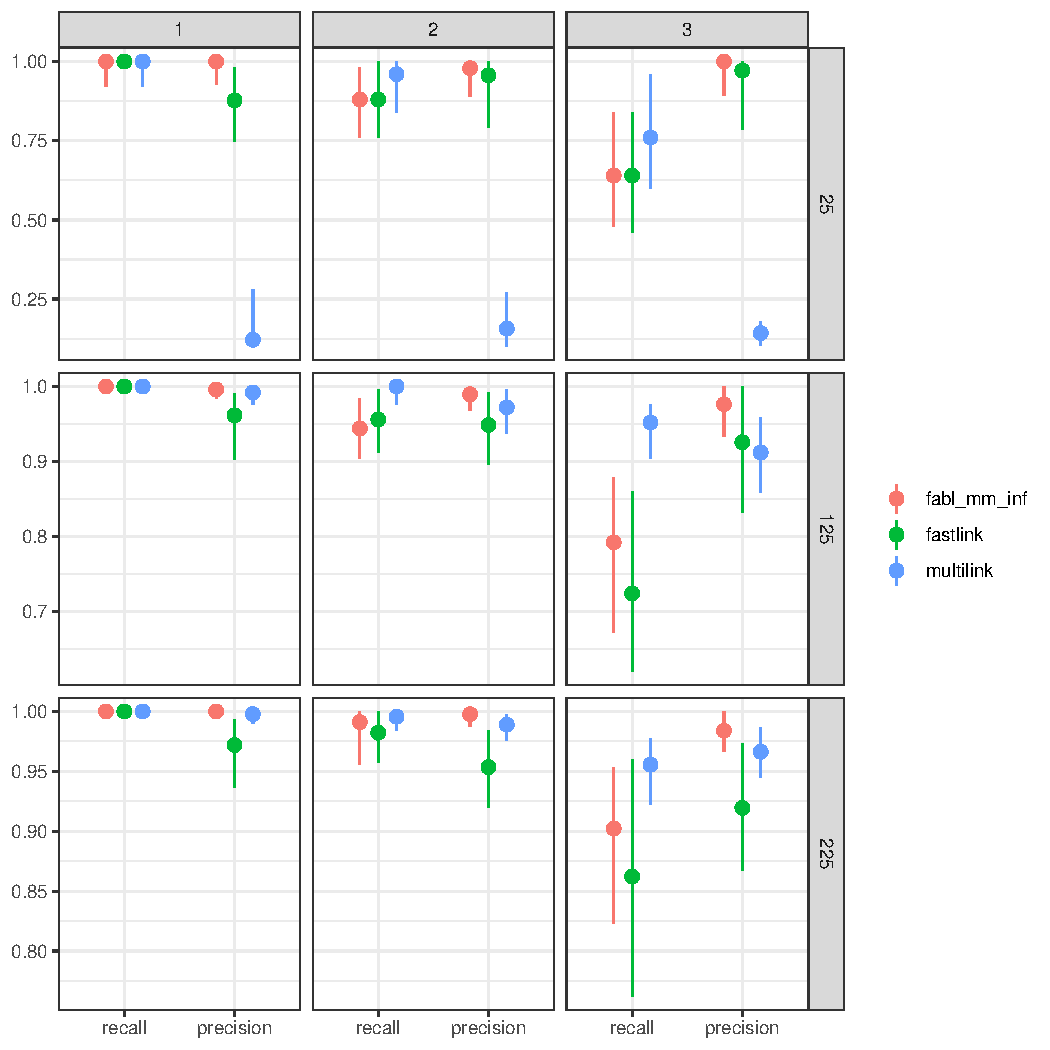
\includegraphics[width=0.8\textwidth]{../Rplots.pdf}
%	\caption{Sadinle Simulation}
%	\label{fig:sadinle}
%\end{figure}

\begin{figure}[t]
	\centering
	\includegraphics[width=0.8\textwidth]{../figures/sadinle_recall.png}
	\caption{Recall for simulations in Section~\ref{sec:simulations}.}
	\label{fig:sadinle-recall}
\end{figure}

\begin{figure}
	\centering
	\includegraphics[width=0.8\textwidth]{../figures/sadinle_precision.png}
	\caption{Precision for simulations in Section~\ref{sec:simulations}.}
	\label{fig:sadinle-precision}
\end{figure}

\begin{figure}
	\centering
	\includegraphics[width=0.8\textwidth]{../figures/sadinle_fmeasure.png}
	\caption{F-Measure for simulations in Section~\ref{sec:simulations}.}
	\label{fig:sadinle-fmeasure}
\end{figure}


In these simulations, standard \texttt{fabl} drastically underperforms, so much so we omit results from the figures below. For each record in $B$ with matching records in $A$, the posterior match probability is split between the two matching records. Due to the randomness of the Gibbs sampler, one of the records occasionally has a posterior probability over 0.5 and is thus identified through the Bayes estimate, but often, both records have posterior probability below 0.5. Under \texttt{vabl}, the posterior probability of the two records is cut precisely in half, and thus \texttt{vabl} did not identify any matching record pairs in any of the simulations. Again, these results are omitted.

We see that \texttt{fastLink} generally has poorer performance than the more complex models at mid to high overlap. In particular, without a post-processing step tailors the scenario where one record in $B$ can match to multiple records in $A$, \texttt{fastLink} tends to produce a large number of false positives, hindering precision, as shown in Figure \ref{fig:sadinle-precision}.

The performance of \texttt{multilink} is more varied. When using substantive prior information, \texttt{multilink} outperforms \texttt{DRL} in terms of overall F-measure in the medium and high overlap settings. However, when the number of matching records pairs is low, \texttt{multilink} underperforms. This may be because the model being fit is more complex, and so it is more difficult to learn the parameters from such few observations. Notably however, the performance of \texttt{multilink} is highly sensitive to prior specification. When using default settings, \texttt{multilink} showed considerably lower recall and precision at all levels of error and overlap.



%The "fabl swap" approach here is also strong. It generally has higher recall, but lower precision. This makes sense, because it doesn't need to consecutive matching algorithim in order to find the "multiple matches", but it also doesn't employ any post processing to clean up erroneous matches. In all simulations, multiple match and fabl swap have similar f-measure. (Not sure exactly how I want to analyze that. In NCVR, there is more of a difference.) 

We see that \texttt{DRL} is a strong alternative to \texttt{multilink} and \texttt{fastLink} in this setting. \texttt{DRL} maintains strong performance even in the low overlap scenario where \texttt{multilink} fails, and outperforms \texttt{fastLink} in terms of F-measure at all levels of error and overlap. We accomplish this through default, uniform priors for the sequence of $\eta_k$ parameters, without needing the informative priors required for \texttt{multilink}. Additionally, the average computation time for 1000 iterations of the Gibbs sampler for \texttt{DRL} was around 30 seconds, while it was around 1000 seconds for \texttt{multilink}. 

\section{Case Study}\label{sec:case-study}

We demonstrate our method on the North Carolina Voter Registration (\texttt{NCVR}) database taken two months apart ~\citep{christen_preparation_2014}. The snapshots are filtered to include only those voters whose details changed over the two-month period, so there are matching records with full agreement on all fields. We use first name, middle name, last name, as string fields, and street address and age as categorical fields. Unique voter registration numbers are provided, however they are known to contain some errors. The \texttt{NCVR} dataset is not publicly available due to sensitive information. However, we have permission to utilize it for publication by its owner.

Using the voter registration numbers, we can see that each file has internal duplication rates of about 1\%. In this analysis, we deduplicate file $B$, and left $A$ with duplicates. In practice, such low amount of internal duplication may not warrant the use of Dirichlet Beta Linkage since \texttt{vabl} is considerably faster. However, we demonstrate here that even with such few internal duplications, \texttt{DRL} is effective at identifying this multiple matches and does not declare too many false matches. 

I compare four approaches: standard \texttt{fabl}, our proposed \texttt{DRL} method, \texttt{fastLink}, and \texttt{fastLink} with the Jaro correction. This task is too large for running \texttt{multilink} in its current implementation in \texttt{R}, and is thus omitted. For \texttt{fastLink}, we use the threshold of 0.5 to declare matches, and for \texttt{fabl} and \texttt{DRL}, we use losses that are equivalent to a threshold of 0.5. Results are in Table \ref{table:ncvr_results}.

\begin{table}[t]
	\centering
	\begin{tabular}{l|rrr}
		method & recall & precision & f\_measure\\
		\hline
		\texttt{DRL} & 0.9891623 & 0.9735309 & 0.9812843\\
		\hline
		\texttt{fabl} & 0.9743739 & 0.9798799 & 0.9771191\\
		%\hline
		%fabl\_swap & 0.9842840 & 0.9420737 & 0.9627164\\
		\hline
		\texttt{fastLink} & 0.9988472 & 0.8494865 & 0.9181321\\
		\hline
		\texttt{fastLink} (with Jaro) & 0.9514490 & 0.9664229 & 0.9588775\\
	\end{tabular}
	\caption{Accuracy results for \texttt{NCVR}, showing the \texttt{DRL} has the highest f-measure.}
	\label{table:ncvr_results}
\end{table}

We see that \texttt{fastLink} without the one-to-one post-processing results in the highest recall, but leads to an undesirable amount of false positives. Since the posterior match probability of each record pair is computed independently, we expect such behavior on large linkage tasks such as this. When we use the Jaro post-processing to achieve a one-to-one matching, we get considerably better results. However, we lose the possibility of identifying cases where one record in $B$ matches to two records in $A$, and we still have worse recall and precision than attained under standard \texttt{fabl}. 

In Figure~\ref{fig:ncvr_thresholds}, we show the show the precision, recall, and F-measure under various choices of match probability thresholds. We see that \texttt{fabl} and \texttt{DRL} produce more refined match probability estimates, allowing the accuracy metrics to vary smoothly across the different thresholds. In contrast, all record pairs of the same agreement pattern under \texttt{fastLink} have the same posterior probability, leading to much a much coarser posterior distribution, leading to more erratic curves. We see that \texttt{fabl} maintains the highest precision at all thresholds, but that \texttt{DRL} is able to identify enough more additional true matches that \texttt{DRL} maintains the highest overall F-measure.
%Overall, we see that \texttt{DRL} has the highest F-measure under all probability thresholds considered, followed by \texttt{fabl}, and then by \texttt{fastLink}.
\begin{figure}[t]
	\centering
	\includegraphics[width=0.9\textwidth]{../figures/ncvr_thresholds}
	\caption{Accuracy metrics for NCVR data at various match probability thresholds. We see that \texttt{DRL} maintains the strongest F-measure for all thresholds considered.}
	\label{fig:ncvr_thresholds}
\end{figure}

Lastly, we note a limitation in using preexisting software for record linkage tasks. In its currently implementation, \texttt{fastLink} allows users to define normalized Levenshtein distance thresholds for coding field comparisons into three discrete levels. In this data however, it is common for a record to contain a middle initial (like ``E"), rather than a full middle name (like ``Elizabeth"). Using Levenshtein distance thresholds, the comparison field for middle name for such a pair of records could coded as a full disagreement, when it should be more reasonably given its own agreement level. Likewise, when two records have a middle initial that happens to match, this is coded as a full agreement, even though it is possible these initials represent different names. In this analysis, 27.6\% of the false matches under \texttt{DRL} at the 0.5 probability threshold included at least one record containing a middle initial rather than middle name. A more careful construction of the comparison vectors is likely to improve results for all methods considered.

\section{Conclusion}\label{sec:conclusion}

In \cite{kundinger_2024_vabl}, we showed how the \texttt{fabl} model could be fit through variational inference, resulting in variational beta linkage, or \texttt{vabl}. As variational inference is much faster than MCMC methods, we showed that \texttt{vabl} was 50-250 times faster than \texttt{fabl} in a number of simulations and case studies. Unfortunately, it is infeasible to fit the \texttt{DRL} model directly through variational inference, since the joint distribution of all possible combinations of records in $A$ is far too high dimensional to estimate without the use of the sequential sampler. However, if we set a limit for the number of matches for each record in $B$, and use stringent blocking criteria to reduce the set of possible combinations of matches, variational inference may be of use in this scenario as well. 
\brian{I think this is probably too specific. Just typing it out as  brainstorm for what to put here.}
%\section{Loss Function}
%
%If we assume there are no duplicates in the base file.
%
%In other Bayesian record linkage approaches, researchers have proposed specialized loss functions that match the specific record linkage model. \cite{sadinle_bayesian_2017}
%
%
%To obtain an estimate $\hat{\bm{Z}}$ of the linkage structure, we use the loss functions and Bayes estimate from \cite{sadinle_bayesian_2017}. Since we model the set of matches for each record $B_j$ independently, it is possible for this Bayes estimate to violate transitivity requirements. Formally, all matched sets such that $\hat{Z}_j \cap \hat{Z}_{j'} = \emptyset$ or  $\hat{Z}_j \cap \hat{Z}_{j'} = \hat{Z}_j$ are in concordance with transitivity. In contrast, 
%
%To obtain a Bayes estimate that fulfills the bipartite requirement, we minimize the expected loss subject to the constraint that $\hat{Z}_j \neq \hat{Z}_{j'}$ for all $j \neq j'$. See Supplement \ref{bayes-estimate} for details regarding the initial Bayes estimate and this post-processing procedure.
%
%If we know that there are no duplication in $B$, we can use the same loss function that we used in \texttt{fabl}. Of course, if we know there are no duplications, we can always swap the datasets and use standard \texttt{fabl} instead of the more complicated multiple match. 
%
%If there are potentially duplicates within $B$, then we need a different loss function to preserve transitivity. One idea is a slightly altered version of the I'm using maximal matching sets from \cite{steorts_bayesian_2016}.
%
%$$p(Z_j = q) =  \frac{1}{S}\sum_{s = 1}^S I\left(Z_j^{(s)} = q\right)$$
%
%Maximal matching sets are in conflict if one is a strict (or proper) subset of another. That is, the matching sets $Z_j$ and $Z_{j'}$ are in conflict if $Z_j \subsetneq Z_{j'}$ or $Z_{j'} \subsetneq Z_j$. In such cases, we calculate the total probability for each cluster, given by $|\hat{Z}_j| p(Z_j = q)$, and accept cluster with the highest total probability. This post-processing ensures transitivity. 



%\subsection{Variational Inference}
%There are several reasons why this prior would not be practical through variational inference.
%\begin{itemize}
%	\item Through MCMC, we can sequentially sample all plausible matches for record $B_j$. In variational inference however, we need to estimate the match probability for the joint distribution of ever possible combination of matches. 
%	\item Without hashing, the number of possible combinations is $n_A \choose k$. With hashing, this number is $P^k / k!$ (I think), and would still require some operations at the scale of $n_A \choose k$ when conducting the actual hashing.
%	\item However, this approach might work if using aggressive indexing/filtering.  
%\end{itemize}
%In cases where we know at least one file is duplicate free, we can safely use \texttt{vabl}. However, if we want to be cautious about the potential for duplicates, the multiple match prior under \texttt{fabl} is a good option. 

%\subsection{Computational Considerations}
%We can set the maximum number of linkages per record, $K$, or let it be estimated by the model. Setting it ahead of time gives a minor (I would say, negligible) computational advantage over leaving it unrestricted. 
%
%Let $L_k^{(s)}$ be the number of records in $B$ with at least $k$ links in $A$ during iteration $s$ of the Gibbs sampler. Note that $L_0 = n_B$ and $L_1 = n_{12}(Z^{(s)})$ when conducting single matching. The computational complexity of multiple match using MCMC is $\mathcal{O} \left(P \sum_{k=0}^K L_k\right)$.
%
%When $X_1$ is free of duplicates, the multiple match algorithm makes a second attempt at matching, which has complexity $ \left(P L_1 \right)$. This is a minor addition of computation time, but gives the added security of identifying duplicates. It may be a nice option just to use when you're not sure!

%
%The "fabl swap" approach here is also strong. It generally has higher recall, but lower precision. This makes sense, because it doesn't need to consecutive matching algorithim in order to find the "multiple matches", but it also doesn't employ any post processing to clean up erroneous matches. In all simulations, multiple match and fabl swap have similar f-measure. (Not sure exactly how I want to analyze that. In NCVR, there is more of a difference.) 
%
%We see that multiple match is a strong alternative to multiple match in this setting. In particular, the average computation time for 1000 iterations of the Gibbs sampler for multiple match was around 30 seconds, while it was around 1000 seconds for \texttt{multiple match}. 
%
%\begin{figure}[t]
%	\centering
%	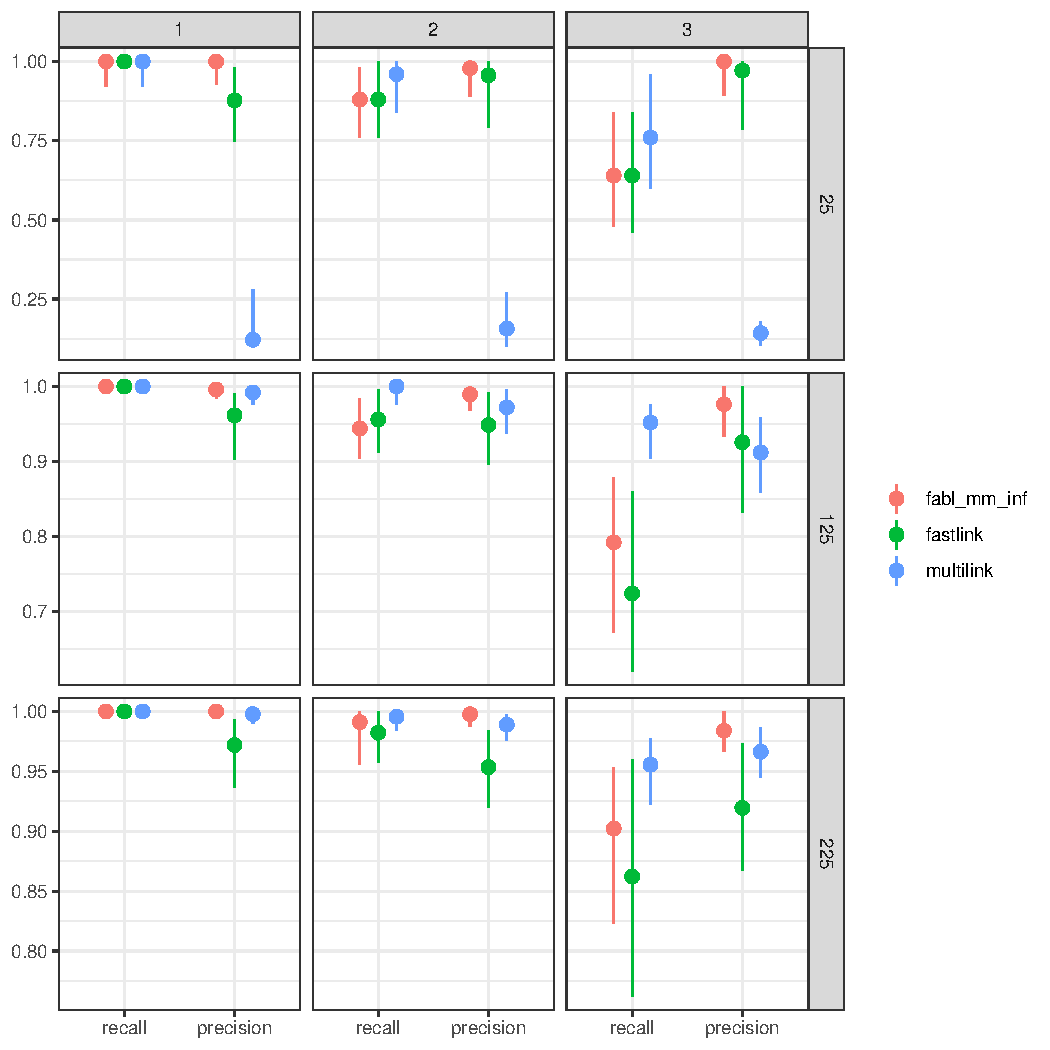
\includegraphics[width=0.8\textwidth]{../Rplots.pdf}
%	\caption{Sadinle Simulation}
%	\label{fig:sadinle}
%\end{figure}
%
%
%NOTE: I've included fastlink (without Jaro) in this image for the time being. However, there is currently no way through fastlink to produce estimates that respect the 2-to-1 matchings while enforcing transitivity. 
%


%We conduct linkage when matching records exhibit 1, 2, and 3 errors across the four fields, and when there are 25, 125, and 225 records in $B$ that have matching records in $A$. To test  Under each of these settings, we use 100 pairs of simulated data files in order to obtain uncertainty quantification on our performance metrics.

%The simulations employ a collection of synthetic data files with varying amounts of error and overlap (the number of records in common across files). Following methods proposed by \cite{christen_pudjijono2009} and \cite{christen_vatsalan2013}, clean records are first simulated from frequency tables for first name, last name, age, and occupation in Australia. Fields are then chosen for distortion uniformly at random. Names are subject to string insertions, deletions and substitutions, as well as common keyboard, phonetic, and optical recognition errors. Age and occupation are distorted through keyboard errors and missingness. These synthetic data files are available in the supplement to \cite{sadinle_bayesian_2017}.
%
%We create comparison vectors according to the default settings of the \texttt{compareRecords} function from the \texttt{BRL} package, shown in Table \ref{Tab:sadinle_simulation_cutoffs}. Each simulation identifies matched individuals between two data files, each with 500 records. We conduct linkage when matching records exhibit 1, 2, and 3 errors across the four fields, and when there are 50, 250, and 450 individuals in common across data files. Under each of these settings, we use 100 pairs of simulated data files in order to obtain uncertainty quantification on our performance metrics. We use uniform priors for the $\bm{m}$, $\bm{u}$, and $\pi$ parameters, with $\alpha_{fl} = \beta_{fl} = 1$ for all $f$ and $l$. We run the Gibbs sampler for 1000 iterations, and discard the first 100 as burn-in. We calculate Bayes estimates $\hat{\bm{Z}}$ of the linkage structure using the  loss function and post-processing procedure described in Supplement \ref{bayes-estimate}. Traceplots for parameters of interest for one example simulation are provided in Supplement \ref{app:appendix-sim}; they show no obvious concern over MCMC convergence. We also replicate this simulation allowing \texttt{fabl} to leave some components of the linkage structure undetermined and left for clerical review; those results are in Supplement \ref{partial}.


%Show accuracy under various settings of maximum cluster size for different algorithms. Recall will fall very quickly for \texttt{fabl}. Since we can't use Jaro, precision for \texttt{fastLink} will be poor.  Multilink may be very dependent on correctly specifying $K$. This multiple match approach should remain strong in all settings. 

\pagebreak
\bibliographystyle{agsm}
\bibliography{biblio}

\pagebreak

\section{Appendix}
\label{sec:appendix}

\subsection{Full Conditional for $Z_j$}\label{app:joint-distribution}

Following the observation of \cite{wortman2019} and elaborated by \cite{kundinger_2023}, when $B_j$ does not link to any record in $A$ (such that $|Z_j| = 0$) the contribution to the likelihood is simply a product of $u$ parameters, which we will call $c_j$:
\begin{align}
	p(\Gamma_{.j}| \bm{m}, \bm{u}, \pi, Z_j = \emptyset) = \prod_{i=1}^{n_A}\prod_{f=1}^{F}\prod_{l=1}^{L_f} u_{fl}^{I(\gamma_{ij}^f = l)I_{obs}(\gamma_{ij}^f)} = c_j.
\end{align}
When $Z_j = q =  (q_1, \ldots, q_k)$ for some $|q| > 0$, we have
\begin{align}
	p(\Gamma_{.j}| \bm{m}, \bm{u}, \pi,  Z_j = q) =\prod_{i \in q}\prod_{f=1}^{F}\prod_{l=1}^{L_f} m_{fl}^{I(\gamma_{ij}^f = l)I_{obs}(\gamma_{ij}^f)}  \prod_{i \notin q}\prod_{f=1}^{F}\prod_{l=1}^{L_f} u_{fl}^{I(\gamma_{ij}^f = l)I_{obs}(\gamma_{ij}^f)}.
\end{align}
We multiply and divide by the $u$ parameters for the matching record pairs to obtain
\begin{align}
	p(\Gamma_{.j}| \bm{m}, \bm{u}, \pi, Z_j = q) &= \prod_{i \in q}\prod_{f=1}^{F}\prod_{l=1}^{L_f} \left(\frac{m_{fl}}{u_{fl}}\right)^{I(\gamma_{ij}^f = l)I_{obs}(\gamma_{ij}^f)}  \prod_{i = 1}^{n_A}\prod_{f=1}^{F}\prod_{l=1}^{L_f} u_{fl}^{I(\gamma_{ij}^f = l)I_{obs}(\gamma_{ij}^f)} \\
	&= c_j \prod_{i \in q} w_{ij} .
\end{align}

Lastly, we multiply the likelihood by the prior in (\ref{eqn:z}) to obtain the posterior distribution. For $Z_j = q$ where $|q| = k$, we have
\begin{subequations}
	\begin{align}
		p\left(Z_j  = q|\gamma, \bm{m}, \bm{u}, \pi \right) &= \frac{\frac{(n_A - k)!|k|!}{n_A!} \pi_{k} c_j \prod_{i \in q} w_{ij}}{\sum_{h \in \mathcal{Z}} \frac{(n_A - |h|)!|h|!}{n_A!} \pi_{|h|} c_j \prod_{i \in h} w_{ij}} \\
		&= \frac{\frac{(n_A - k)!|k|!}{n_A!} \pi_{k} \prod_{i \in q} w_{ij}}{\sum_{h \in \mathcal{Z}} \frac{(n_A - |h|)!|h|!}{n_A!} \pi_{|h|} \prod_{i \in h} w_{ij}} \\
		&\propto \frac{(n_A - k)!|k|!}{n_A!} \pi_{k} \prod_{i \in q} w_{ij}.
	\end{align}
\end{subequations}

\subsection{Derivation of Sequential Sampler}\label{app:sequential-sampler}
We now provide the derivation of the sequential sampler, following the argument presented in Section \ref{sec:joint-distribution}. Suppose $B_j$ has been linked to $k$ records in $A$. Let $Z_{j, -k} = (Z_{j, 1}, \ldots, Z_{j, k-1})$ denote the vector of records already linked to $B_j$. When $B_j$ has no additional link in $A$, the contribution to the likelihood is a product of the $u$ parameters for all remaining records. That is, 
\begin{align}
	p(\Gamma_{.j}| \bm{m}, \bm{u}, \pi, Z_{j, k} = \emptyset, Z_{j, -k} = q_{-k}) = \prod_{i \notin Z_{j, -k}} \prod_{f=1}^{F}\prod_{l=1}^{L_f} u_{fl}^{I(\gamma_{ij}^f = l)I_{obs}(\gamma_{ij}^f)} = c_{Z_{j, -k}}.
\end{align}

When $Z_{j, k} = q_k$ for some $q_k > 0$, we have
\begin{align}
	p(\Gamma_{.j}| \bm{m}, \bm{u}, \pi,  Z_{j, k} = q_k, Z_{j, -k} = q_{-k}) &=\prod_{f=1}^{F}\prod_{l=1}^{L_f} m_{fl}^{I(\gamma_{q_k, j}^f = l)I_{obs}(\gamma_{q_k, j}^f)}  \prod_{i \notin (q_{-k}, q_k)}\prod_{f=1}^{F}\prod_{l=1}^{L_f} u_{fl}^{I(\gamma_{ij}^f = l)I_{obs}(\gamma_{ij}^f)} \\
	&=\prod_{f=1}^{F}\prod_{l=1}^{L_f} \left(\frac{m_{fl}}{u_{fl}} \right)^{I(\gamma_{q_k, j}^f = l)I_{obs}(\gamma_{q_k, j}^f)}  \prod_{i \notin (Z_{j, -k}}\prod_{f=1}^{F}\prod_{l=1}^{L_f} u_{fl}^{I(\gamma_{ij}^f = l)I_{obs}(\gamma_{ij}^f)} \\
	&= c_{Z_{j, -k}} w_{q_k, j}
\end{align}
To obtain the posterior, we multiply by the prior in (\ref{eqn:sequential_prior}). The posterior distribution this is given by
\begin{align}\label{eqn:sequential-posterior-full}
	p(Z_{j, k} = q_k|Z_{j, k-1}, \eta_k, \bm{m}, \bm{u}, \gamma) &=
	\frac{\left(\frac{\eta_k}{n_A - (k - 1)}c_{Z_{j, -k}} w_{q_k, j}\right)^{I(q_k \in N_{j, k})} + \left(c_{Z_{j, -k}}(1 - \eta_k)\right)^{I(q_k = \emptyset)}}{\frac{\eta_k}{n_A - (k - 1)}c_{Z_{j, -k}} \sum_{i \notin Z_{j, -k}} w_{ij} + c_{Z_{j, -k}}(1 - \eta_k)} \\
	&=
	\frac{\left(\frac{\eta_k}{n_A - (k - 1)}w_{q_k, j}\right)^{I(q_k \in N_{j, k})} + (1 - \eta_k)^{I(q_k = \emptyset)}}{\frac{\eta_k}{n_A - (k - 1)}\sum_{i \notin Z_{j, -k}} w_{ij} +(1 - \eta_k)} \\
	&\propto \begin{cases}
		\frac{\eta_k}{n_A - (k - 1)} w_{q_k, j}, & q_k \in N_{j, k}, \\
		1 - \eta_k, & q_k= \emptyset.
	\end{cases}
\end{align}
Importantly, the constant $c_{Z_{j, -k}}$ is not found in the final expression because the probability mass associated with every potential value for $Z_j$ shares the same $c_{Z_{j, -k}}$. This does not occur due to proportionality. 


%\subsection{Extended Proof} \label{app:extended-proof}
%\begin{align*}
%	p\left(Z_j  = q |\gamma, \bm{m}, \bm{u}, \pi\right) &\propto \frac{(n_A - |q|)!|q|!}{n_A!} \pi_{|q|} \prod_{i \in q} w_{ij} \\
%	&= \prod_{c = 1}^{|q|} \frac{1}{n_A - (c + 1)} (1 - \eta_{|q|+1}) |q|!\prod_{c = 1}^{|q|} \eta_{|q|} \prod_{c = 1}^{|q|} w_{q_c, j} \\
%	&= (1 - \eta_{|q|+1}) |q|!\prod_{c = 1}^{|q|} \frac{\eta_{|q|} }{n_A - (c + 1)}  \prod_{c = 1}^{|q|} w_{q_c, j} \\
%	&= p(Z_{j, |q|+1} = \emptyset| \eta_{|q|})|q|! \prod_{c = 1}^{|q|} p(Z_{j, c} = q_c|\eta_c) p(\Gamma_{.j}| \bm{m}, \bm{u}, \bm{\eta}, q_c \in Z_j) \\
%	&\propto p(Z_{j, |q|+1} = \emptyset | \Gamma_{.j}, \bm{m}, \bm{u}, \bm{\eta}) |q|!\prod_{c = 1}^{|q|} p(Z_{j, c} = q_c|\Gamma_{.j}, \bm{m}, \bm{u}, \bm{\eta}).
%\end{align*}
%
%\begin{align}
%	p\left(Z_j  = q|\gamma, \bm{m}, \bm{u}, \pi \right) &= \frac{\frac{(n_A - |q|)! |q|!}{n_A!} \pi_{|q|} c_j \prod_{i \in q} w_{ij}}{\sum_{h \in \mathcal{Z}} \frac{(n_A - |h|)! |h|!}{n_A!} \pi_{|h|} c_j \prod_{i \in h} w_{ij}} \\
%	&= \frac{\frac{(n_A - |q|)! |q|!}{n_A!} \pi_{|q|} \prod_{i \in q} w_{ij}}{\sum_{h \in \mathcal{Z}} \frac{(n_A - |h|)! |h|!}{n_A!} \pi_{|h|} \prod_{i \in h} w_{ij}} \\
%	&\propto \frac{(n_A - |q|)! |q|!}{n_A!} \pi_{|q|} \prod_{i \in q} w_{ij}
%\end{align}
%
%\begin{align}
%	\prod_{c = 1}^{|q|} p\left(Z_{j, c} = q_c|\gamma, \bm{m}, \bm{u}, \eta_c, Z_{j, c-1} \right) &=  (1 - \eta_{|q|+1}) |q|!\prod_{c = 1}^{|q|} \frac{\eta_{|q|} }{n_A - (c + 1)}  \prod_{c = 1}^{|q|} w_{q_c, j}
%\end{align}


\subsection{Efficient Sequential Sampling Details}
%Following \cite{kundinger_2023} we use hashing to reduce the computational complexity of the Gibbs sampler. Since each component $\gamma_{ij}^f$ of the comparison vector is discrete, there are only finitely many possible realizations of the comparison vector $\gamma_{ij}$. Let $P$ be the number of unique agreement patterns observed in $\Gamma$. This number is bounded above by $P^{*} =  \prod_{f=1}^F (L_f + 1)$, where the addition of 1 to $L_f$ for each field accounts for the possibility of missing values. This upper bound does not scale with $n_1$ or $n_2$, but rather is determined by $F$ and $L_f$.  
%
%We adopt a hashing function to map the $P$ unique agreement patterns present in the comparison vectors to the integers in $[P]$. Let
%\begin{equation}
%	\label{eq:hashfunc}
%	h_f^{(i,j)} = I_{obs}( \gamma_{ij}^f) 2^{\gamma_{ij}^f + I(f>1) \times \sum_{e=1}^{f-1}(L_{e} - 1)}
%\end{equation}
%denote a hashed value for field $f$ for record pair $(i,j)$. Summing over the fields for the agreement pattern of record pair $(i,j)$ gives the hash value $h^{(i,j)}=\sum_{f=1}^Fh_f^{(i,j)}$. We enumerate the unique hashed agreement patterns from $1$ to $P$. Denote each agreement pattern as $h_p=(h_p^1,\dots,h_p^F)$, so that when record pair $(i,j)$ exhibits agreement pattern $p$, we write $\gamma_{ij}=h_p$.  Collect the agreement patterns as $\mathcal{P}=\{h_p\mid p\in[P]\}$.
%
%Let $e(h_p)$ denote the $\sum_{f=1}^FL_f$ length vector in which the $l + \sum_{k=1}^{f-1} L_k$ component is 1 when $h_p^f = l$, and 0 otherwise. Observe that $e(h_p)$ represents a long version of $h_p$, which is useful for computational purposes. Let $N_{p_j}=\sum_{i=1}^{n_2}I(\gamma_{ij}=h_p)$ denote the number of records in $X_1$ with which record $j$ in $X_2$ has agreement pattern $p$. Collect these counts in $\mathcal{N}=\{N_{p_j}\mid j\in[n_2], p\in[P]\}.$ Let $N_p=\sum_{j=1}^{n_2}N_{p_j}$ denote the total number of record pairs with agreement pattern $p$. Finally, let $r_{p_j}=\{i\in[n_1]\mid \gamma_{ij}=h_p\}$ be the set of records in $X_1$ with which record $j$ in $X_2$ has agreement pattern $p$, and collect these sets as $\mathcal{R}=\{r_{p_j}\mid p\in[P], j\in[n_2]\}$. 
%
%The set $\tilde{\bGamma}=\{ \mathcal{P}, \mathcal{R},\mathcal{N}\}$ fully characterizes the information in $\bGamma$ at a reduced storage cost. In particular, by letting 
%\[
%m_p = \prod_{f=1}^F\prod_{l=1}^{L_f} m_{fl}^{I(h_p^{f}=l)I_{obs}(h_p^{f})}
%\]
%and
%\[
%u_p = \prod_{f=1}^F\prod_{l=1}^{L_f} u_{fl}^{I(h_p^{f}=l)I_{obs}(h_p^{f})},
%\]
%the likelihood function in \eqref{eqn:likelihood} can be written as
%\begin{equation}
%	\label{eq:likelihoodhash}
%	\mathcal{L}(Z, m,u\mid\tilde{\Gamma})=\prod_{j=1}^{n_2}\prod_{p=1}^{P}\prod_{i\in r_{p_j}}m_p^{I(Z_j=i)}u_{p}^{I(Z_j\neq i)}.
%\end{equation} 
\subsection{Bayes Estimate}\label{app:bayes-estimate}

\end{document}
